\subsection{Hardware eval}
In order to verify the correctness of our hardware designs, we have created gate-level implementations of them compatible with the pulse transfer simulator PyLse \cite{pylse}.
The gate models we used are mostly based on the open source RSFQ cell library from Sun Magnetics \cite{rsfqlib} with the addition of a few cells we tuned ourselves, like the Muller C and inverted C elements.
Using these models, we run extensive testing by comparing the measured outcomes of our circuits for thousands of randomly sampled inputs to the results predicted by higher order models.
An example simulation in Figure~\ref{fig:pylserun} shows the pulses in the data input ($x$) and select output ($sel$) wires of a small arbiter selecting the two largest priority scores out of four ($k=2,n=4$).
We used a small number of operands for this simulation in order to keep the plot interpretable.
These simulations additionally provide accurate numbers for the latency and JJ count of various circuit components.
These results are shown in Table~\ref{tab:arbstats} and Table~\ref{tab:encoderstats}.
As shown in these tables, the area cost for generating priority scores is fairly low for each logical qubit at only a few thousand JJs, and the overhead of the arbiter stays at the order of tens of thousands when managing many logical qubits ($n=256$).
This hardware cost is low enough to make our design viable for today's limited integration density, which is the largest roadblock for hardware meant to operate at the 4 Kelvin environment.
Additionally, the combined delay of both priority score generation and the arbiter barely crosses the nanosecond mark for the largest sizes considered, which is negligible compared to the total decoding time.



\begin{table}[]
\caption{Area and delay measurements for arbiters supporting various numbers of logical qubits.}
\label{tab:arbstats}
\begin{tabular}{|l|l|l|l|}
\hline
k & n   & JJ count & latency (ps) \\ \hline
2 & 64  & 6971     & 379          \\ \hline
4 & 128 & 25793    & 588          \\ \hline
8 & 256 & 83345    & 847          \\ \hline
\end{tabular}
\end{table}

\begin{table}[]
\caption{Area and delay measurements for complex flag generation (CPX) and encoding to priority score (ENC).}
\label{tab:encoderstats}
\begin{tabular}{|l|l|l|l|l|}
\hline
d  & CPX JJ cost & ENC JJ cost & CPX latency & ENC latency \\ \hline
3  & 176         & 390         & 95          & 143         \\ \hline
5  & 592         & 430         & 105         & 157         \\ \hline
7  & 1244        & 490         & 109         & 164         \\ \hline
9  & 2132        & 570         & 116         & 171         \\ \hline
11 & 3256        & 670         & 116         & 171         \\ \hline
13 & 4616        & 790         & 119         & 174         \\ \hline
15 & 6212        & 930         & 119         & 174         \\ \hline
17 & 8044        & 1090        & 126         & 181         \\ \hline
19 & 10112       & 1270        & 126         & 181         \\ \hline
21 & 12416       & 1470        & 126         & 181         \\ \hline
\end{tabular}
\end{table}

\begin{figure}
  \begin{center}
    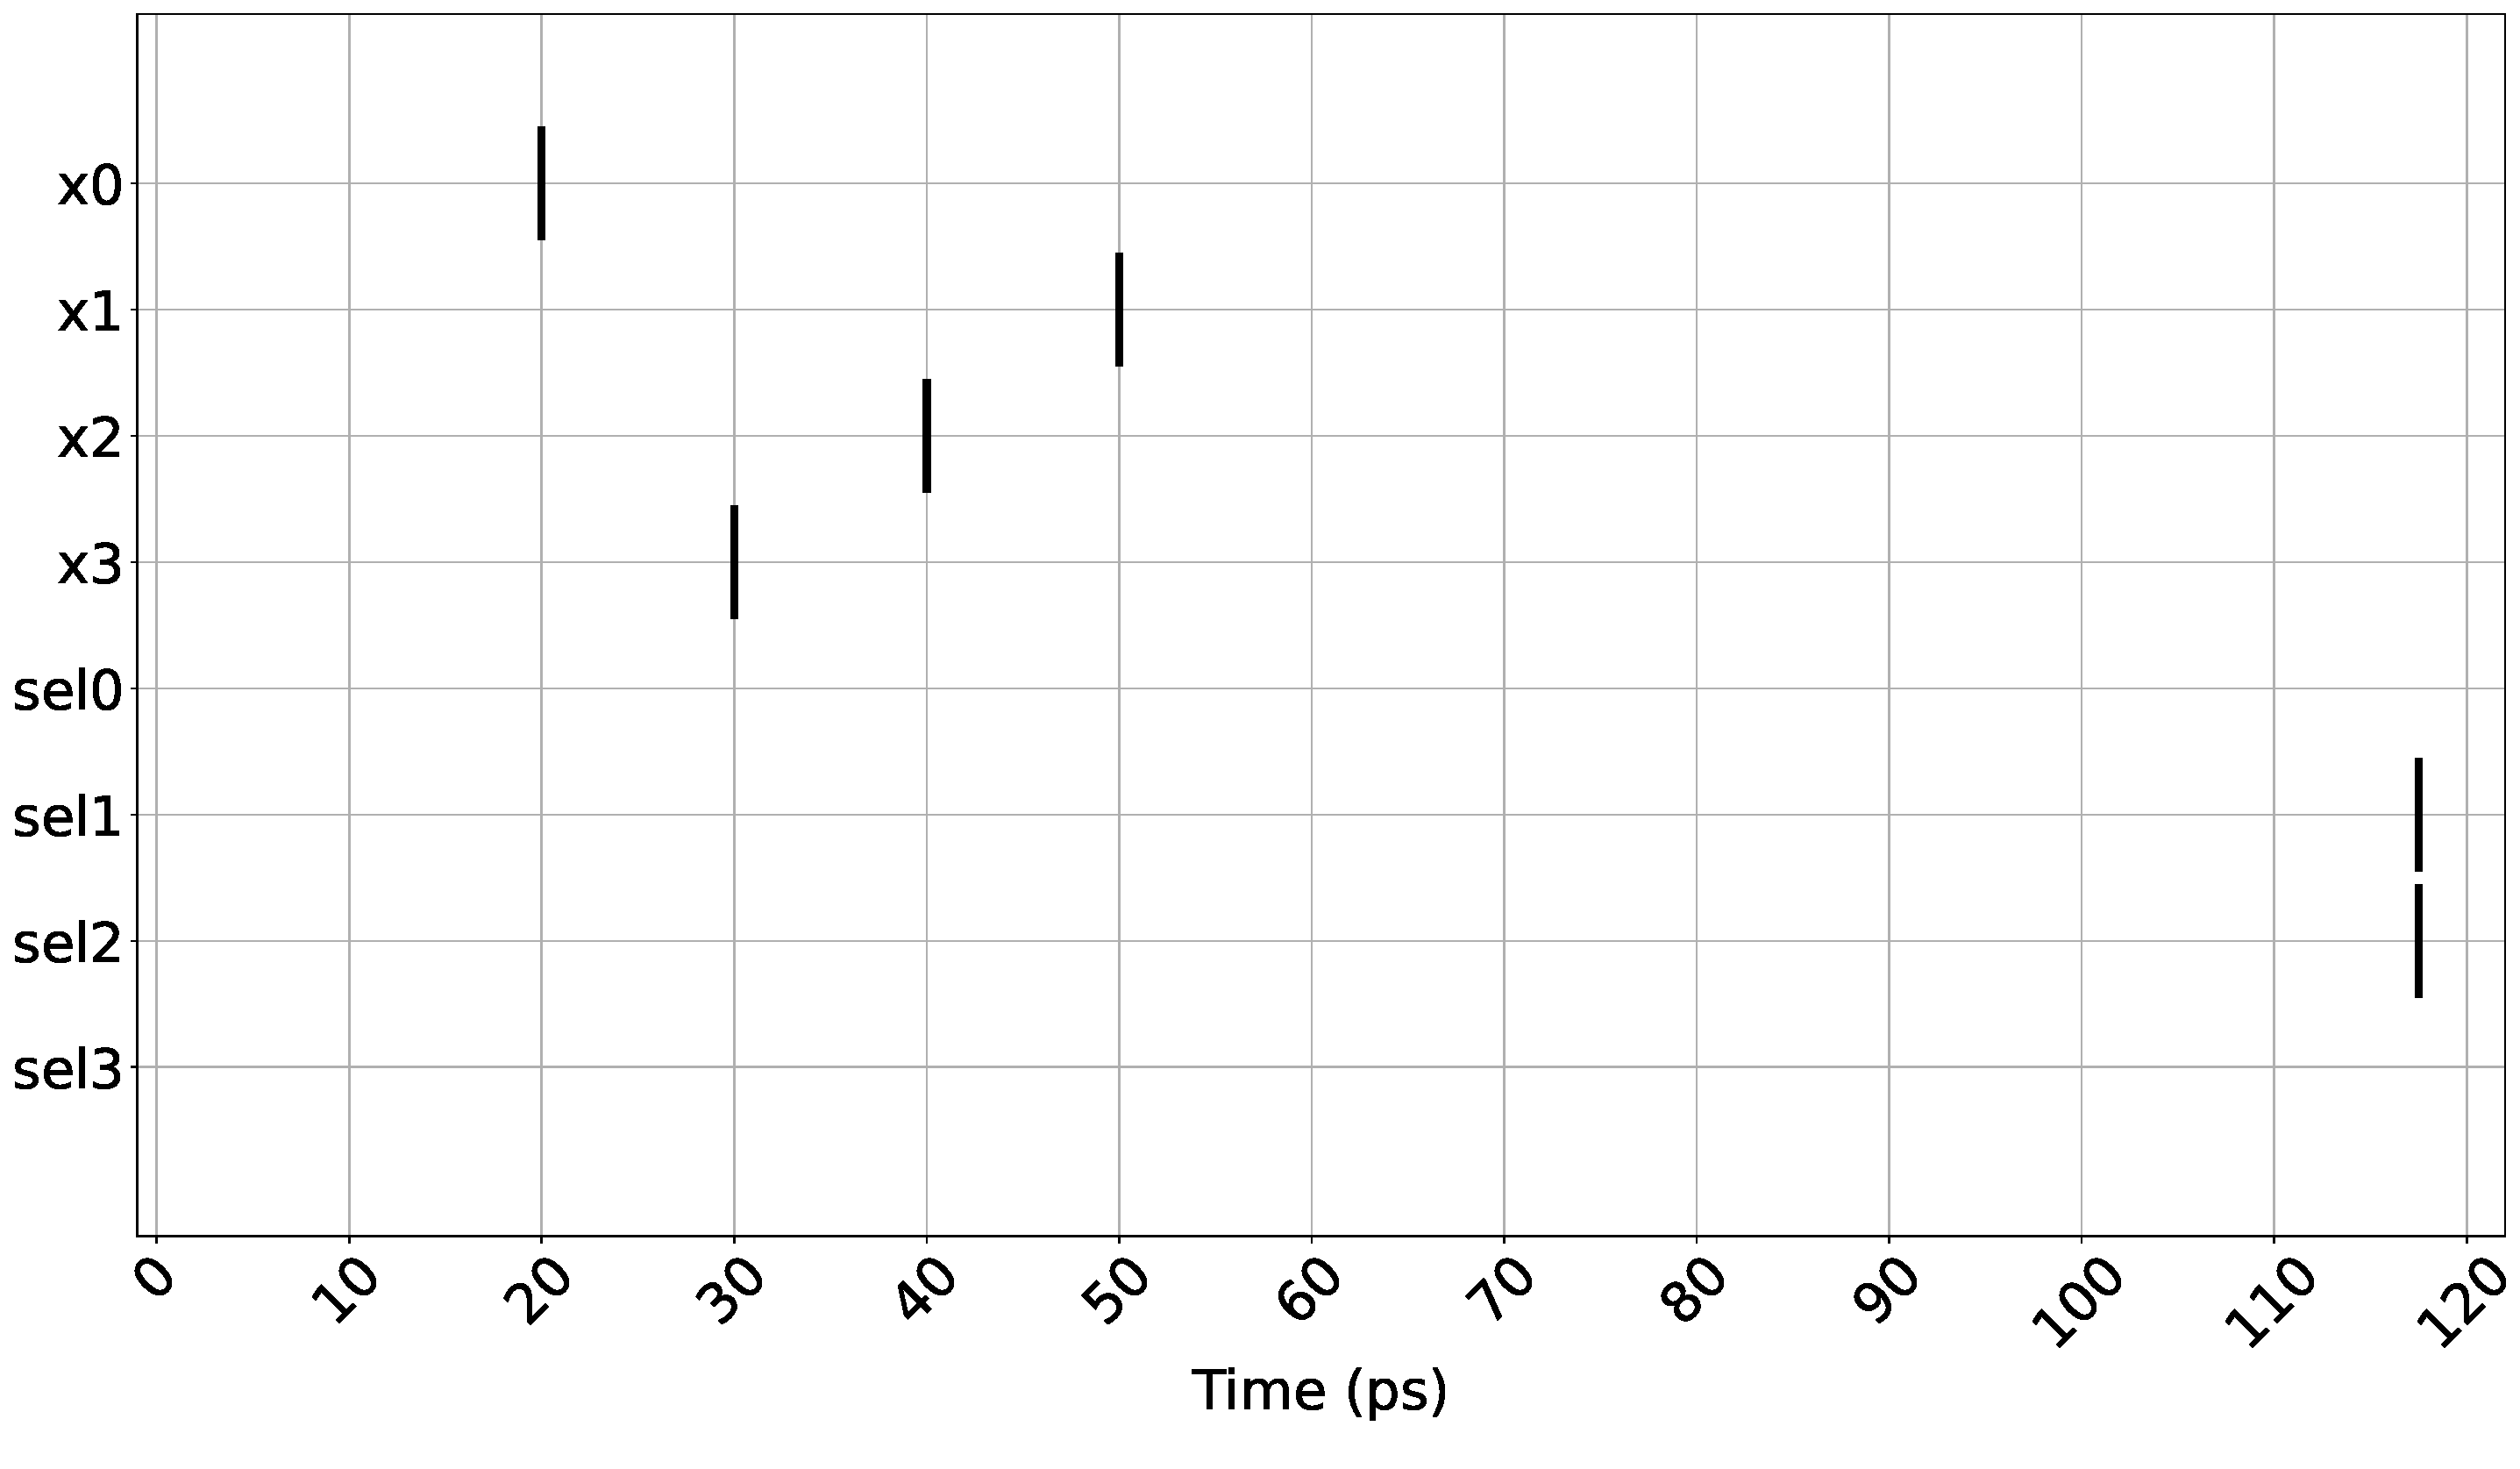
\includegraphics[width=\columnwidth]{figures/arbi.pdf}
  \end{center}
  \caption{}\label{fig:pylserun}
\end{figure}

